\documentclass{article}\usepackage[]{graphicx}\usepackage[]{color}
%% maxwidth is the original width if it is less than linewidth
%% otherwise use linewidth (to make sure the graphics do not exceed the margin)
\makeatletter
\def\maxwidth{ %
  \ifdim\Gin@nat@width>\linewidth
    \linewidth
  \else
    \Gin@nat@width
  \fi
}
\makeatother

\definecolor{fgcolor}{rgb}{0.345, 0.345, 0.345}
\newcommand{\hlnum}[1]{\textcolor[rgb]{0.686,0.059,0.569}{#1}}%
\newcommand{\hlstr}[1]{\textcolor[rgb]{0.192,0.494,0.8}{#1}}%
\newcommand{\hlcom}[1]{\textcolor[rgb]{0.678,0.584,0.686}{\textit{#1}}}%
\newcommand{\hlopt}[1]{\textcolor[rgb]{0,0,0}{#1}}%
\newcommand{\hlstd}[1]{\textcolor[rgb]{0.345,0.345,0.345}{#1}}%
\newcommand{\hlkwa}[1]{\textcolor[rgb]{0.161,0.373,0.58}{\textbf{#1}}}%
\newcommand{\hlkwb}[1]{\textcolor[rgb]{0.69,0.353,0.396}{#1}}%
\newcommand{\hlkwc}[1]{\textcolor[rgb]{0.333,0.667,0.333}{#1}}%
\newcommand{\hlkwd}[1]{\textcolor[rgb]{0.737,0.353,0.396}{\textbf{#1}}}%
\let\hlipl\hlkwb

\usepackage{framed}
\makeatletter
\newenvironment{kframe}{%
 \def\at@end@of@kframe{}%
 \ifinner\ifhmode%
  \def\at@end@of@kframe{\end{minipage}}%
  \begin{minipage}{\columnwidth}%
 \fi\fi%
 \def\FrameCommand##1{\hskip\@totalleftmargin \hskip-\fboxsep
 \colorbox{shadecolor}{##1}\hskip-\fboxsep
     % There is no \\@totalrightmargin, so:
     \hskip-\linewidth \hskip-\@totalleftmargin \hskip\columnwidth}%
 \MakeFramed {\advance\hsize-\width
   \@totalleftmargin\z@ \linewidth\hsize
   \@setminipage}}%
 {\par\unskip\endMakeFramed%
 \at@end@of@kframe}
\makeatother

\definecolor{shadecolor}{rgb}{.97, .97, .97}
\definecolor{messagecolor}{rgb}{0, 0, 0}
\definecolor{warningcolor}{rgb}{1, 0, 1}
\definecolor{errorcolor}{rgb}{1, 0, 0}
\newenvironment{knitrout}{}{} % an empty environment to be redefined in TeX

\usepackage{alltt}
\usepackage{float}
\usepackage{graphicx}
\usepackage{tabularx}
\usepackage{siunitx}
\usepackage{mdframed}
\usepackage{cite}
\usepackage{natbib}
\bibliographystyle{..//refs/styles/besjournals.bst}
\usepackage[small]{caption}
\setkeys{Gin}{width=0.8\textwidth}
\setlength{\captionmargin}{30pt}
\setlength{\abovecaptionskip}{0pt}
\setlength{\belowcaptionskip}{10pt}
\topmargin -1.5cm        
\oddsidemargin -0.04cm   
\evensidemargin -0.04cm
\textwidth 16.59cm
\textheight 21.94cm 
%&\pagestyle{empty} %comment if want page numbers
\parskip 0pt
\renewcommand{\baselinestretch}{1}
\parindent 20pt
\usepackage{multirow}
\newmdenv[
  topline=true,
  bottomline=true,
  skipabove=\topsep,
  skipbelow=\topsep
  ]{siderules}
%\usepackage{lineno}
%\linenumbers
\IfFileExists{upquote.sty}{\usepackage{upquote}}{}
\begin{document}
\title{Phenological sensitivity as a mediator of plant interactions}
\author{Dissertation proposal of Daniel Buonaiuto}
\maketitle{}
\section*{Motivation and Dissertation Framework}
\indent\indent Phenology, the timing of annual life cycle events, allows organisms to synchronize important life history transitions with optimum environmental conditions \citep{Forrest2010}. Phenology is an important mediator of ecosystem processes \citep{Piao2007,Cleland2007} and species interactions \citep{Yang2010,Leverett2017}, and plays a major role in determining species' range limits \citep{Chuine2001}. Pronounced shifts in phenology observed across a broad range of taxa have been reported, with plant phenology shifting by 3-5 days on average per decade \citep{Parmesan2003,Menzel2006,Root2003}. Phenological sensitivity to climate change varies among taxa, and there is evidence that within given communities species phenologies are shifting at different rates \citep{Cleland2012,Ovaskainen2013}. These differential sensitivities are likely to have far reaching effects on community interactions, but our ability to predict these second order effects remain limited.
\par In my proposed dissertation, I heed this call to advance our understanding of the effects of global change on species interactions as mediated through phenology. Sitting at the nexus of traditional community ecology and global change biology, my proposed dissertation will explore 1] how differences in sensitivity to environmental conditions can produce significantly different phenological patterns and 2] how differential phenological responses alter community interactions.
\par In \textbf{Chapter I}, I use experimental manipulations and statistical modeling to evaluate the currently evolutionary hypotheses regarding flower-leaf phenological sequences in temperate woody plant species, and investigate differential phenological sensitivity between flower and leaf buds as a potential mechanism for this variability.
\par In \textbf{Chapter II}, I turn my attention to seed germination phenology, where I probe the effect of variable stratification periods and incubation temperature on germination of a large suite of temperate, herbaceous plants, to determine interspecific differences in responses to changing climate, and evaluate the likelihood of germination rank changes under future climate scenarios.
\par In \textbf{Chapter III}, I expand the scope of my inquiry in chapter II, compiling a global database of experimentally manipulated germination trials, and use meta-analysis techniques to better understand the reaction norm of germination phenology in response to environmental manipulations.
\par In \textbf{Chapter IV}, I perform a direct test of the impact of phenological shifts on community interactions, by using alternate climatic treatment to manipulate the germination phenologies of two species growing in a pairwise competition experiment.

\section*{Background}
\indent\indent\textbf{Eco-physiology and Evolution of Spring Phenology:} Plants sense and interpret a complex set of environmental cues that signal the changing of the seasons and can respond by fine-tuning their phenological transitions accordingly \citep{Vitasse2010}. For plants growing in temperate regions, it is widely accepted that phenological transitions are responses to the interaction of exogenous environmental conditions, temperature and photoperiod \citep{Forrest2010}, with endogenous cues like circadian clocks \citep{Visser2010}. Temperature and light are also considered to be the main drivers of seed germination \citep{Finch-Savage2006}. In the temperate zone, both seeds and buds generally cycle through a state of dormancy, a temporary state in which metabolic activity is minimized, preventing organism growth, development or activity. Dormancy allows organisms to persist by conserving energy during periods that are unfavorable for biological functioning, which in the temperate zone, is the cold months of winter. There is a complicated taxonomy of dormancy in seeds \citep{Baskin2004}, and the most common dormancy class in the temperate regions of the world is physiological dormancy (PD), in which a physiological inhibition mechanism is present in the embryo and prevents radical emergence \citep{Finch-Savage2006}. While globally, there are several climactic factors that contribute to dormancy break, in our region, this transition from dormancy to growth tends to be mediated by exposure to a prolonged period of cool temperatures (chilling or stratification), followed by warm (forcing or incubation) temperatures. It should be noted that the first visible sign that dormancy is broken is germination or budburst, so as such, it is difficult, and even controversial, to mark where dormancy ends and growth begins \citep{Long2015,Bewley1997}.
\par The same selective forces determining the optimum timing for transition from dormancy to growth have been suggested for both spring germinating seeds and bud phenology. The adaptive benefits of early phenological transition, an extended growing season, predator avoidance, and reduced competition for resources are balanced by the higher risk of mortality due to biotic and abiotic factors \citep{Rathcke1985}. For flower buds, the availability of pollinators may be an additional selection factor. As such, the phenological optimum evolves in relation to other functional traits and life history tradeoffs. 
\par While the selective forces, environmental conditions and conceptual framework for the transition from dormancy to growth may be quite similar for seeds and buds, there is evidence that the physiological mechanisms regulating these processes are quite different. In buds, short day conditions and the end of the season induce dormancy by isolating meristematic cell interactions through heavy deposits of callose in the plasmodesmata\citep{Rinne2011,Sager2014}. Winter chilling degrades the callose, reengaging cellular integration for the transition to growth under suitable conditions. 
\par In seeds, Abscisic acid (ABA), a hormone up-regulated during seed maturation is generally thought to initiate and maintain dormancy as its concentration tends to decrease as seeds approach germination \citep{Baskin2014, Fenner2000}. Environmental treatments such as cold or warm stratification and afterrippening, have been shown to contribute to the degradation of ABA, and an upregualtion and increased sensitivity to the growth hormone gibberelic acid ($GA_3$), as well as ethylene and brassinosteroids, which promotes germination \citep{Kucera2005}.

\textbf{Model of Spring Phenology:} Many models have been developed to use temperature to predict phenology in woody plants \citep{Chuine2002}, while seed science most commonly uses a single model, the thermaltime or cardinal temperature model, or its variant the hydrothermaltime model which includes water potential as a parameter\citep {Bradford2002}.The thermaltime model of germination describe the relationship between time, temperature and germination fraction at sub-optimal temperatures.\\

\theta_{T}(g)=(T-T_{b})t_{g}\\

where $\theta_{T}(g)$ is thermal time to gemination, T is the treatment temperature, $T_b$ is the base temperature below which germination rate is 0 and $t_g$ is the time to a given germination fraction. If not observed experimentally, $T_b$ can be inferred through statistical methods by regressing the reciprocal of germination time against a given germination fraction and determining the x-intercept \citep{Pritchard1999}.
If supra-optimal temperature are included in the experiment, which would be indicated by a reduction in germination rate at higher temperatures, a constant $K_t$ is added to the equation to modify the thermal time parameters by the following equation:\\

\theta_{T}=(k_{T}(T-T_{o}))(T-T_{b})t_{g}\\

where $T_o$ is the optimum temperature.
\par While this model is widely toted for its biological accuracy in predicting the germination phenology of non-dormant seeds \citep{Bradford2005}, the standard thermaltime model is less effective for phenological predictions with dormant species \citep{Batlla2015}.
\par Several attempts have been made to modify this modeling framework to better incorporate a dormancy module. Conceptually, dormancy break treatments reduce $T_b$ or($psi_b$ in the hydrothermaltime variant) allowing for a more rapid accumulation of thermaltime and more rapid germination. This framework has been applied to include afterrippening \citep{Meyer2000}, and cold stratification\citep{Pritchard1996,Batlla2003}, but has not been broadly applied outside of agriculture or horticulture, and its effectiveness for a diversity of taxa remains unknown \citep{Steadman2004}. By evaluating the change in germination rate at different dormancy break treatment, one can determine a coefficient which reflects the rate of change in $T_b$. The equation is formulated below:\\

$T_b= (\beta(t_s))+T_b(o)$\\

where $\beta$ is constant rate of decline, $t_s$ is the stratification time, and $T_b(o)$ is the base temperature without dormancy treatment.

\section*{chapter I: The significance of flower-leaf sequences in an era of global climate change}
\subsection*{Introduction}
\indent\indent Why do some tree species seasonally flower before leafing out? This sequence, known as hysteranthy, proteranthy, or precocious flowering is readily apparent in many ecologically and commercially important species and has been described as  the characteristic flower-leaf sequence (FLS) of temperate deciduous forests \citep{Rathcke1985}. Most of the current hypotheses regarding FLS's suggest that they critical to the reproductive or physiological functioning of woody plants \citep{Gougherty2018}. Several authors suggest that the hysteranthous FLS is a trait critical for wind-pollination efficiency \citep{Whitehead1969,Friedman2009}. Others suggest that flowering first is an adaptation to reduce water stress and maintain floral hydration \citep{Franklin2016}, though this hypothesis has emerged primarily from the dry-deciduous tropics where hysteranthy is also common \citep{Janzen1967,Franklin2016}.  Still others suggest the hysteranthous FLS is an adaptation to allow for extremely early flowering and is correlated with other early flowering traits such as seed size, dispersal time and cold tolerance \citep{Gougherty2018,Bolmgren2003,Primack1987}. It is also possible that FLS's are highly conserved, and the preponderance of hysteranthy in the temperate zone is a product of phylogenetic representation of the region rather than an adaptive quality to the trait.\\
\indent Despite the rich theoretical attention FLS has received in the literature, data about FLS is limited. The most comprehensive source of data we have regarding FLS comes from categorical, qualitative descriptions in regional flora and guide books. A few long term empirical datasets in which FLS can be properly described as a continuous variable can be found, but these are rare, as flower and leaf phenology have generally been treated and observed separately \citep{Wolkovich2014}. In part I of this chapter I ask, given the available data:
\begin{enumerate}
\item  What is the association between FLS and several other life history traits (pollination syndrome, shade tolerance, plant height, flowering time, duration of fruit maturation) pertinent to the established hypotheses? Are these results sensitive to data quality, observational ambiguity and modeling choices? Does treating FLS as a continuous rather than categorical variable change the model inference?
\end{enumerate}
\indent\indent Treating FLS as a categorical trait masks important characteristics of FLS such as the range variability of FLS offset between species, individuals, populations and years. As far as I know, there have been no attempts to empirically quantify this variability. Improving our understanding of the variability of this pattern would aid significantly in evaluating the evolutionary hypotheses for FLS, and serve to generate hypotheses for the eco-physiological mechanisms behind these patterns. In part II of this chapter I ask:
\begin{enumerate}
\item What is the range in variability in FLS between species, years and individuals?
\item Is variability in FLS a product of differential sensitivities to environmental cue combinations between flower and leaf buds?
\end{enumerate}

\subsection*{Methods:}
\indent\indent\textbf{Part I:} I obtained species level descriptions of floral-foliate sequences and trait information from the regional guidebook Michigan Trees \citep{Barnes2004} and its companion volume Michigan Shrubs and Vines \citep{Barnes2016} (hereafter: MTSV) and the Unites States Forest Services Silvic Manual Vol.2 \citep{Burns1990} (hereafter: USFS). All categorical traits were reclassified as binary (FLS, shade tolerance, pollination syndrome). I developed two, alternative classifications for FLS, physiological (only taxa with ``flowers before leaves" hysteranthous) and functional (taxa with ``flowers before leaves", ``flowers before/with leaves" and ``flowers with leaves" considered hysteranthous). In total, 196 and 82 woody species, in MTSV and USFS respectively, were included in my analysis. To investigate the phylogenetic signal of hysteranthy and control for phylogenetic structure in the datasets, I used a published angiosperm phylogenetic tree \citep{Zanne2013} pruned to match the species list from the MTSV and USFS data. Species not in the tree were added at the generic root. I used  a generalized linear modeling framework \citep{Ives2010} to build a logistical regression model corrected for phylogenetic structure using the R package phylolm \citep{Ho2014}. The model was run with 599 bootstrapped re-sampling iterations for each dataset \citep{Wilcox2010}. Continuous predictors were rescaled by subtracting the mean and dividing by two standard deviations to allow for a reasonable comparison of effect sizes between the binary and continuous predictors in this model \citep{Gelman2007}. Models were run on each dataset for each classification of FLS for sensitivity analysis.\\ 
\indent For the model with FLS as a continuous response, I used a long term phenological dataset from Harvard Forest in Petersham, MA \citep{Okeefe2015} (hereafter: HAFO)  and calculated the average FLS lag time for 21 species which overlapped the MTSV species list. With the same modeling framework, I modeled the associated between the original MTSV predictors and the Harvard forest continuous FLS data.\\
\indent\textbf{Part II:} I first determined descriptive statistics (mean, standard deviation and range) and plotted the seasonal dynamics of FLS offset in the HAFO dataset using the R base statistical package to establish a basic understanding of the typical variability in FLS. In October of 2017, I obtained cutting of dormant twigs from 12 woody plant species from Harvard Forest in Petersham MA. Twigs were transported to the Weld Hill Research Building in Boston, MA, re-cut in water, and placed into 250 ML Erlenmeyer flasks. 6 replicates of each species were randomly assigned to different growth chamber temperature and photoperiod combinations. Twigs received 1 of 2 levels of chilling (4 or 8 weeks at 4 degrees), combined with 1 of 2 forcing treatments (24/18 or 18/12 day/night temperatures on 12 hour cycles) and 1 of 2 photoperiod treatments (8/16 or 12/12 day/night) for a 12 way full factorial design. Flasks were moved between chambers every 2 weeks to reduce the influence growth chamber effect artifacts on the results. Twigs were monitored for flower and leaf phenology using the bbch scale \citep{Finn2007} every 2-3 days for four months.
\par I currently  use a multilevel, Bayesian, survival analysis framework to analyze these data. Survival analysis is the appropriate framework for this experiment as there was a considerable number of twigs that did not burst buds by then end of the experiment, but were determined to be living. Dead twigs, or those which were determined to have had no flower buds at the outset of the experiment are excluded from the analysis. I predict that the FLS offset will vary significantly between treatment combinations and that this variation will be traceable to flowering and leaf phenology being differentially sensitive to the environmental factors. My initial model is a varying slope/intercept model by species with the following predictor and response formulation:\\
\\
$D_e$ \Leftarrow $\beta_1(photoperiod:phase)+\beta_2(chill:phase)+\beta_3 (force:phase) $\\

Where $D_e$ is the days from initation in forcing conditions to phenological event, and the interaction between phase and each predictor will reveal differences in response to the treatments between floral and leaf phenophases.\\
\subsection*{Status and Preliminary Results:}
\indent\indent\textbf{What is the association between FLS and several other life history traits?  Are these results sensitive to data quality, observational ambiguity and modeling choices?:} In the categorical models, only flowering time is a consistently strong predictor of FLS, with the effect size of pollination syndrome, seed development time and phylogenetic signal varying in significance depending on data source and modeling choices. There was no strong signal from height or shade tolerance. See figure~\ref{fig:Figure 1} for effect size plots.
In the continuous model, pollination syndrome was the strongest predictor of FLS, with the effect size of shade tolerance and early flowering being strong and significant as well (see figure~\ref{fig:Figure 2}). These findings lend support to the pollination syndrome, early flowering hypotheses. It is not surprising that multiple hypotheses find support in this analysis, as FLS is a complex trait that may have developed independently in different selection environments.
\par\textbf{Is variability in FLS a product of a differential sensitivity to environmental cue combinations between flower and leaf buds?:} As seen in the  example plots of \textit{Quercus rubra} phenology at Harvard Forest,(figure~\ref{fig:Figure 3}), there is considerable interannual and inter-individual variation in FLS. Additionally, for this species, there appears to be a temporal trend in which FLS has shifted towards a hysteranthous pattern over time. This phenomenon could be correlated with climate change, and should be investigated further.
\par Preliminary analysis of my experimental result confirms there is considerable variability in FLS offset in different environments see figure~\ref{fig:Figure 4}.  There seems to be support for the hypothesis that this variability is a product of differential sensitivity between flowering and leafing (note in particular, COMPER (\textit{Comptonia peregrina}) and CORCOR (\textit{Corylus cornuta}), in figure~\ref{fig:Figure 5}), but because of many non-response values in the data spread unevenly across species and treatments, this finding has low confidence and other modeling approaches need to be attempted. Below I present other modeling frameworks I will attempt:
\begin{enumerate}
\item Rather than modeling flowering and leafing sensitivities as interactions, use offset (as determined in part I) as a response variable.
\item Use a logistic regression framework with phenology as a binary response.
\item Run individual species models for only the species with the most data.
\end{enumerate}

\section*{Chapter II: The germination response to varying stratification regimes of a suite of temperate herbaceous species}
\subsection*{Introduction}
\indent\indent The cold stratification requirement for dormancy release has been identified in a large number of North American temperate plant taxa, and stratification treatments are employed widely in both plant science and industry \citep{Hartmann_2011}. The duration of stratification needs has also been showm to differ between species, ranging from just a few days to many months \citep{Luna2009}, and may vary significantly depending on temperature and between seed populations \citep{Steadman2004}. While cold stratification is commonly found as an experimental treatment in the literature, and has been shown to advance germination, studies which evaluate the germination response across a range of stratification periods or temperatures are more rare \citep{Batlla2009}. As a result, the kinetics of the germination response to variable stratification regimes is poorly characterized in the vast majority of plant species.\\
\indent Cold stratification in the lab, serves as a proxy for the natural exposure to chilling conditions a seed would experience while overwintering in the field. With global climate change, changes to the severity and duration of winter will alter the natural stratification period experienced by seeds \citep{Walck2011}. While winters are generally predicted to be warmer and shorter \citep{IPCC_2014}, the number of days which the stratification conditions are met may increase, decrease, or shift temporally, differentially affecting the germination phenology plant species depending on their geographic position, and the dynamics of their response to temperature \citep{Walck2011}. These shifts in germination may in turn alter plant competition through priority effects \citep{Gioria2018} and plant demography through seed bank dynamics, and multi-trophic interactions.\\
\indent To better predict the effect of warming winters on seed germination, it is imperative to better characterize the germination response to variable stratification regimes for a more broad range of plant species. In this chapter I ask:
\begin{enumerate}
\item How do varying stratification periods effect the germination time courses of plant species?
\item How do stratification periods and incubation temperatures interact in germination time courses?
\item Is the stratification requirement best characterized by an optimum (can seeds get over stratified) or a threshold?
\item To what degree is germination rank between species affected by varying stratification regimes?
\end{enumerate}
\subsection*{Proposed methods}
\indent\indent\textbf{Experimental Protocols:} In the summer of 2018, seeds of 15 temperate Eastern North America herbaceous plant species of both native and non-native origins were procured from plant nursery stock or collections (see table in figure ~\ref{fig:Figure 6}) and dry-stored until the start of the experiment. In mid-August 2018, all seeds were checked for the presence of an embryo using a float test \citep{Baskin2014}, and imbibed in distilled water for 24 hours. Seeds of each species were then randomly divided into cohorts of 15-20, depending on seed availability, and placed onto wetted sterile sand in 8 cm plastic petri dishes. Three replicates of each cohort were then assigned to a combination of stratification duration (10 levels: 0, 10, 20, 30, 40, 50, 60, 70, 80, 100 days) and incubation (2 levels, low temperature: 20 day/10 night or high: 25 day/15 night) treatments, making for a 20 level fully factorial treatment design. For stratification, petri dishes were wrapped in aluminum foil and placed in a germination chamber in the dark at 4 degrees C. At the end of each stratification duration, cohorts were transferred to incubation conditions in growth chambers. Germination fractions were observed every other day for 25 days, and petri dishes were checked regularly and moistened as needed. By measuring the germination fraction over time, I will generate germination time courses for each species and each treatment.\\
\indent\textbf{Statistical analysis:} Using the germination time courses for each species, I will calculate the rate of change for $T_b$ as a function of stratification duration. From these data, I will assess each species sensitivity to stratification, and use this information to predict how germination rank may change under different stratification scenarios. I will also examine whether species with different traits such as life history, habitat requirements, native status, and phylogeny differ in the strength of their response to the environmental treatments.\\
\subsection*{Status/preliminary results}
\textbf{Project Status:} The experimental procedures are underway, and expected to conclude in December 2018.\\
\section*{OEGRES: A meta-analysis of Observed environmental germination responses in experimental settings}
\subsection*{Introduction and Questions:}
\indent\indent Seed germination is a critical life history stage for plant life, and as such, there is a long history, over 2000 years, of germination research \citep{Baskin2014, Fenner2000}. More comptemorary work has produced a large body of literature detailing the germination requirements and dormancy classes for a vast number of species across an array of taxonomic and geographic space. Many comprehensive books and review papers have been written on the subject, and germination research continues at a rapid pace around the globe, but there are still large gaps in our knowledge \citep{Baskin2014}. As mentioned above, our understanding of  kinetics of the germination response to environmental conditions remain in its infancy.  Without a better understanding of a more complete range of germination responses to different environmental states, it is difficult to predict the extent of climate change impact on plant regeneration. While few individual studies systematically investigate responses to a wide range of environmental conditions, the large body of germination literature could be leveraged to this end. In this chapter, I propose a meta-analysis to more broadly address the questions I laid out in chapter II:
\begin{enumerate}
\item How do varying environmental treatments effect the germination time courses of plant species?
\item How do various environmental treatments interact to effect seed germination?
\item Are there any broad patterns in the germination response to variable environmental conditions at the phylogenetic, geographic, or life-history level?
\end{enumerate}
\indent\indent In addition to these fundamental biological question I will also use this project to address several important questions about germination research methodologies including:
\begin{enumerate}
\item Which environmental cues are most commonly manipulated?
\item What treatment levels are most commonly utilized in research, how often are multiple treatment levels applied within one experiment?
\item Do treatments decisions correlate with other factors such as geography, institution, or taxa studied?
\end{enumerate}
\subsection*{Proposed methods:}
\indent\indent Due to the acknowledged importance of temperature in mediating seed dormancy and germination, my primary interest is to evaluate the effects of stratification and incubation treatments on germination, but I intend to also include other environmental factors, such as water status, soil properties, afterripening, and scarification treatments in my analysis.\\
\indent\textbf{Data collection:} I performed a search of the Web of Science database using the keywords "germination" and "stratification", and excluded meeting abstracts, abstracts of published items and proceedings papers. The search returned 1,208 papers. For each paper, I read the abstract, methods and figures to identify studies that fit for inclusion in my analysis.\\
\indent\textbf{Inclusion criteria:} To be included in the study, papers were required to:
\begin{itemize}
\item Report a temporal germination response in addition to a final germination percentage.
\item Manipulate a temperature variable (cold or warm stratification).
\end{itemize}
Papers that were not fully accessible were also excluded from my analysis. 
\par Because of the large volume of papers, I will randomly sample 2000 papers that meet the selection criteria to build a database, using ImageJ to scrape data from the relevant figures. The response variables I will capture include any measurement or index of germination rate as well as final germination percentages. The predictors I capture in addition to the specific environmental treatments in the paper will include:
\begin{itemize}
\item seed provenance (continent, latitude, longitude, altitude, biome)
\item seed age
\item year of collection and maternal environment
\item dormancy class (if applicable)
\item non-environmental treatments (chemical application)
\item life history
\item population native status
\end{itemize}
\indent\indent\textbf{Analysis:} Upon completion of the database, I will use a multilevel, bayesian modeling framework to assess the impact of varying temperature regimes on germination behavior. I intend to run several models with different grouping factors, including taxonomic and regional. I will also query the database to address the methodological questions addressed above.
\subsection*{Project status:}
As of August 16, I have evaluated 610 papers of which 241 were determined fit for inclusion. Assuming this 39.5 percent inclusion rate remains consistent, I expect that 450-500 studies will be fit for inclusion.
\section*{Chapter IV: Seasonal priority effects: Germination phenology as a mediator of plant competition}
\subsection*{Introduction}
\indent\indent Priority effects, a class of interspecific interaction in which the effect of species on one another depends on the order in which they arrive at a site, are a cornerstone of community assembly theory \citep{Fukami2015}. These historical contingencies have been shown to alter the structure and function of communities, driving communities to alternate stable states \citep{Fukami2011}. Recent theory has suggested that it is not just species' arrival times that determine the course of interactions, but significant priority effects can be determined by the phenological differences between species already resident to a site, a subcategory of historical contingency known as seasonal priority effects (SPE) \citep{Wainwright2012}. Like traditional priority effects, SPE's can operate though niche preemption, in which the species with earlier phenology reduce the amount of resources available for species with more delayed phenological activity, or niche modification, in which earlier phenological initiators modify the environment, determining the growth conditions that the later species will experience. While niche modification effects can be facilitative or detrimental, the effects of niche preemption on the later species is always detrimental \citep{Fukami2015}. Most of the evidence for seasonal priority effects, comes from observation studies correlating higher phenological sensitivity (earlier phenology), with competitive dominance or invasion success \citep{Gioria2018}. However early phenology may be associated with other traits associated with superior competitive ability \citep{Dickson2012}, and the strength of priority effects have been shown to vary based on the identities \citep{Cleland2015} and by environment \citep{Kardol2013}.  While some studies have succeeded in experimentally linked seasonal priority effects with competitive dominance \citep{Wainwright2012}, or inferred seasonal priority effects through sequential planting studies \citep{Korner2008}, to my knowledge, the relative strength of SPE's influence on competition between species has yet to have been quantified in any systems. With the evidence for significant interspecific differences in phenological sensitivity to variable climates, it is likely that climate change will alter the germination lag times or even rank between species. If SPE's do indeed significantly mediate species interactions, these phenological shifts would be expected to have strong implications for community dynamics. In this final chapter I ask:
\begin{itemize}
\item What are the effects of varying SPE's on the competitive dynamics between two species in a controlled environment?
\end{itemize}
\subsection*{Proposed Methods}
\indent\indent Based on results from chapter II, I will select two species for a pairwise competition experiment. The two species will be selected based on the following criteria:
\begin{enumerate}
\item They have similar growth requirements and would be likely to be found in the same habitat in nature.
\item Their germination rank changes or the lag between their respective germination phenology shifts by more than 10-15 days given different stratification/incubation combinations.
\end{enumerate}
\indent\indent Seeds of each species will be sown in a soil medium at varying relative and overall densities following a response surface design detailed in \cite{Inouye2001}, (see figure~\ref{fig:Figure 7}). This design has been shown to be the most effective for differentiating between the effects of intra vs. interspecific competition and integrating data with theoretical models of competition.  Replicates of each density will be randomly assigned to two different stratification/incubation regimes that have previously been show to alter the germination rank of the species, thus manipulating the strength of the seasonal priority effects in the competitive system.\\
\indent After the given stratification period and 25 days of incubation, all pots will be transfered to a greenhouse for the duration of the experiment (12 weeks). Every 4 weeks, the height of each plant will be measured and standardized photos of each pot will be taken to allow for an estimation of percent cover of each species. The measurement will be applied for a biomass estimation using models found in \citet{Axmanova2012}. At each measurement interval, 5 plants of each species, not included in the response surface will be measured, harvested, dried and weighed to better calibrate the biomass models. At the conclusion of the experiment, all plants will be harvested, dried and weighed for a final biomass calculation.\\
\indent\textbf{Analysis:} I will use the repeat measures of biomass to calculate and compare the relative growth rate (RGR) \citep{Connolly2005} of each species under the different priority effect manipulations. I predict that first species to germinate in each treatment will have a higher relative growth rate and suppress the growth rate of the second species. If no switch in germination rank is possible, I expect more pronounced priority effect (great lag between germination), to produce a greater differential in relative growth rate than the weaker priority effect treatment.\\  


\section*{Timeline}
\begin{center}
\begin{tabular}{|c|l|}
\hline
Time & Task\\
\hline
\textbf{Fall 2018}& \\
ch.1 & Write article for part 1\\
ch.2 & Complete experiment data collection\\
ch.3 & Complete OEGRES initial inclusion survey\\
ch.4 &  \\
\hline
\textbf{Spring 2019}& \\
ch.1 & Analysis of part 2\\
ch.2 & Data analysis\\
ch.3 & Begin data scraping\\
ch.4 & Select species and treatment for response surface \\
\hline
\textbf{Summer 2019}& \\
ch.1 & Write article for par 2\\
ch.2 & Continue data analysis\\
ch.3 & Continue data scraping\\
ch.4 & Continue preparations for response surface trials \\
\hline
\textbf{Fall 2019}& \\
ch.2 & Continue data analysis\\
ch.3 & Continue data scraping\\
ch.4 & Initiate treatments, begin competition experiment \\
\hline
\textbf{Spring 2020}& \\
ch.2 & Data analysis\\
ch.3 & Data cleaning\\
ch.4 & Continue experiment\\
\hline
\textbf{Summer 2020}& \\
ch.2 & Conclude Data analysis\\
ch.3 & Data cleaning\\
ch.4 & Begin data analysis\\
\hline
\textbf{Fall 2020}& \\
ch.2 & Write article\\
ch.3 & Modeling\\
ch.4 & Continue data analysis\\
\hline
\textbf{Spring 2021}& \\
ch.3 & Continue Modeling\\
ch.4 & Continue data analysis\\
\hline
\textbf{Summer 2021}& \\
ch.3 & Write article\\
ch.4 & Continue data analysis\\
\hline
\textbf{Fall 2021}& \\
ch.4 & Write article\\
\hline
\textbf{Spring 2022}& Defense \\
\hline

\end{tabular}
\end{center}

\bibliography{prop}
\pagebreak

\section*{Figures}

\begin{figure}[here]
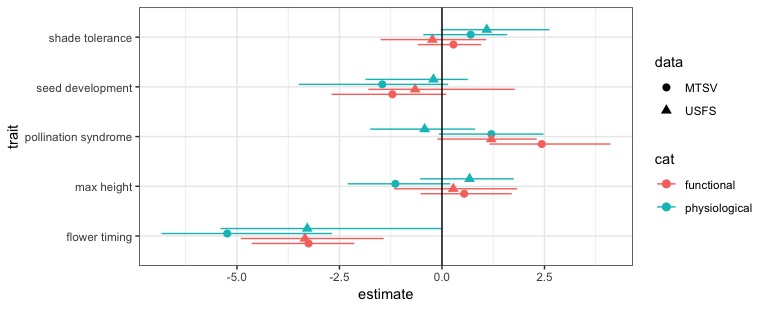
\includegraphics[width=0.9\textwidth]{..//figures/Data_comparision_plot.jpeg}
\caption{Predictor effect size comparisons (means and 95\% bootstrap intervals, scaled predictors) with two different data sources (USFS and MTSV) and two different binary classifications of FLS. Results are sensitive to both data source and modeling choices. }
\label{fig:Figure 1}
\end{figure}

\begin{center}
\begin{figure}[here]
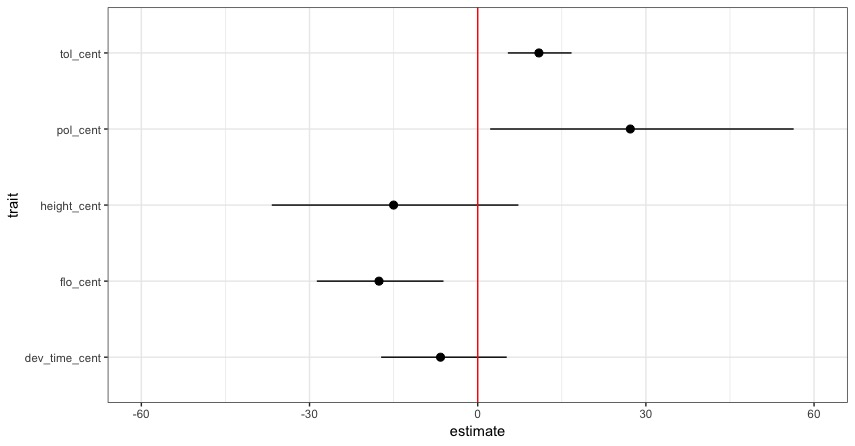
\includegraphics[width=0.9\textwidth]{..//figures/HF_continuous_scaled_mode.jpeg} %remake this figure as a jpeg with better labels
\caption{Model effect sizes (means and 95\% bootstrap intervals) for a model using scaled MTSV predictors with mean FLS offset (in days) for overlapping species from HAFO.}
\label{fig:Figure 2}
\end{figure}
\end{center}

\begin{figure}[here]
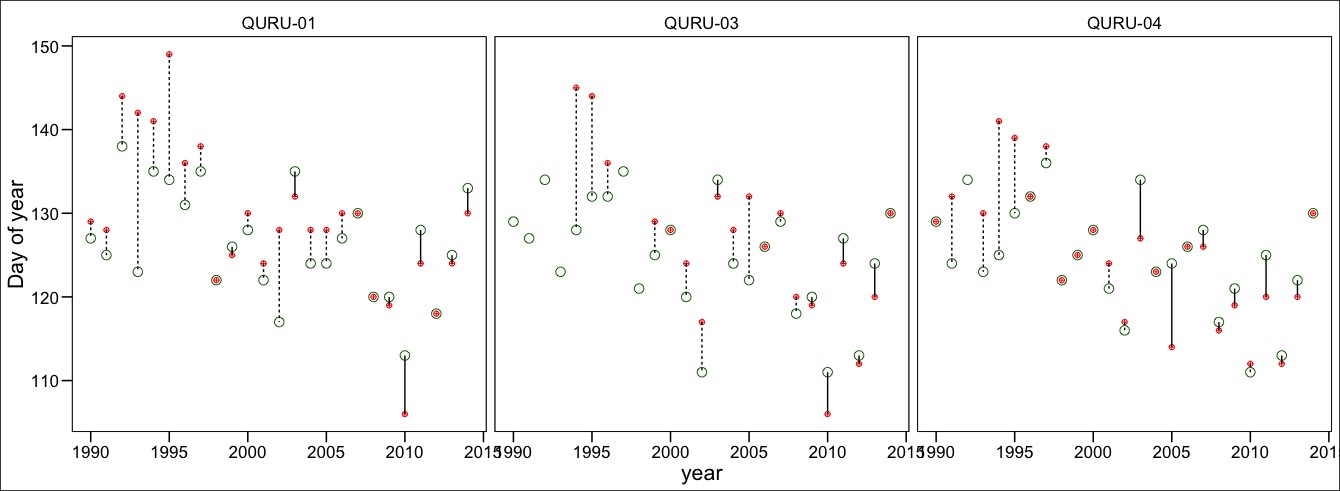
\includegraphics[width=0.95\textwidth]{..//figures/QURU_HF_intervar.jpeg} %remake this figure as a jpeg with better labels
\caption{Plots showing interannual variability in FLS for three \textit{Quercus rubra} indivudals at Harvard Forest from 1990-2015. Red point indicated flower budburst, and green circles leaf budburst. Solid offset lines indicate years of flowering buds bursting first (hysteranthy) and dashed lines indicate years in which leaf buds burst first (seranthy)}
\label{fig:Figure 3}
\end{figure}

\begin{figure}[here]
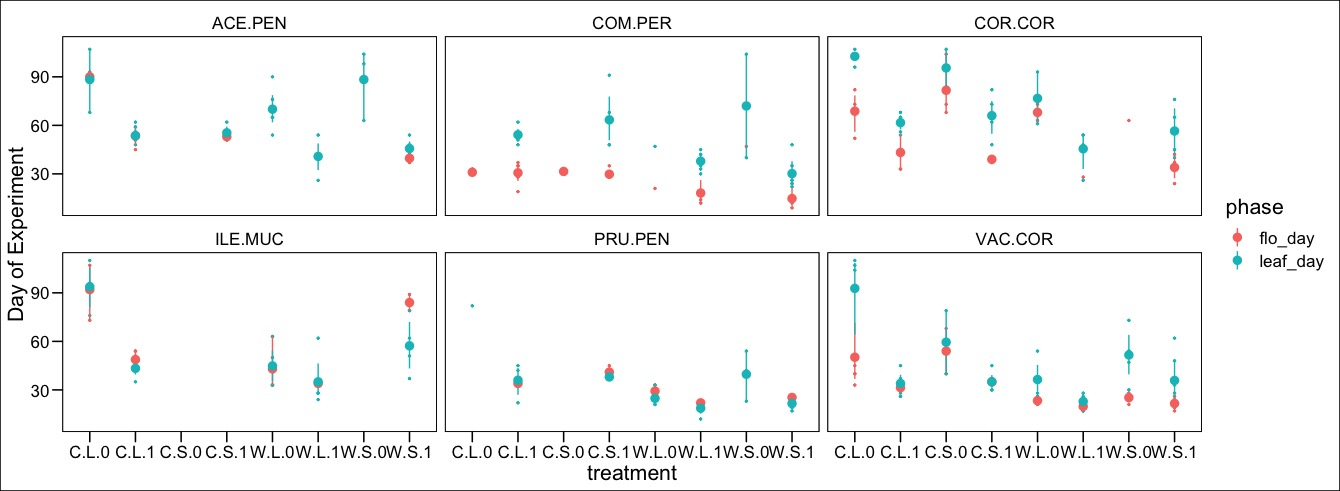
\includegraphics[width=0.95\textwidth]{..//figures/raw_flobuds.jpeg}
\caption{FLS variability (mean and standard deviation flowering and leafout time) for 6 species under different temperature and phtotoperiod regimes.}
\label{fig:Figure 4}
\end{figure}

\begin{figure}[here]
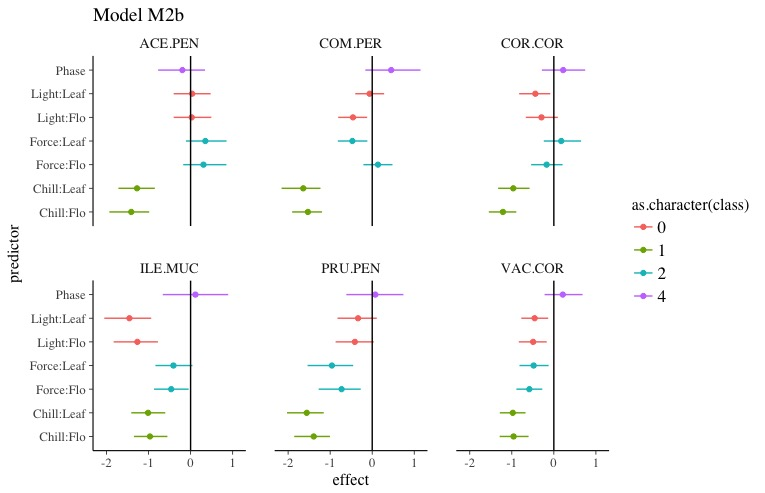
\includegraphics[width=0.8\textwidth]{..//figures/Goods_mod2b.jpeg}
\caption{Effect sizes (mean and 95\% credible intervals for flowering and leafout) of the phenological response to different climatic treatments for flowering and leafout.}
\label{fig:Figure 5}
\end{figure}

\begin{figure}[here]
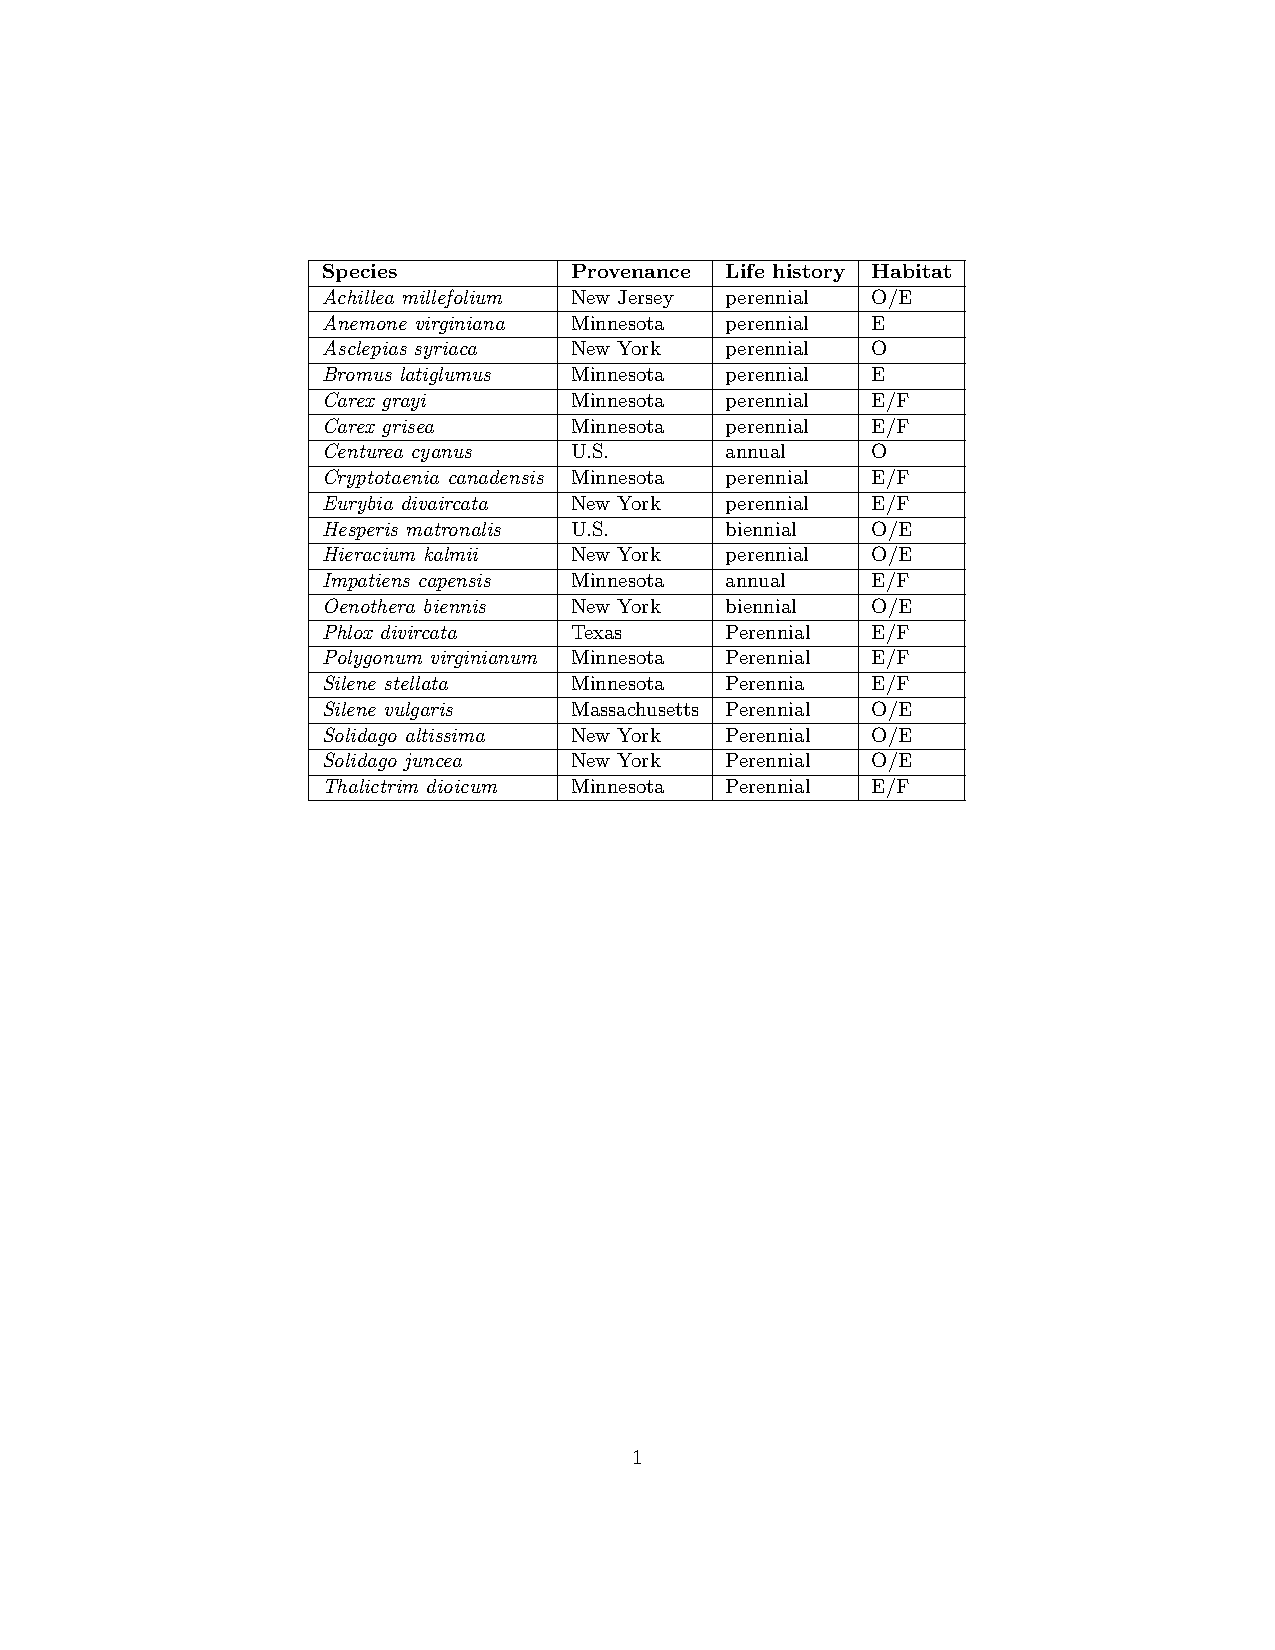
\includegraphics[trim=50 400 50 100,clip,width=0.9\textwidth]{..//figures/species_table.pdf}
\caption{Species information: species, seed provenance, life history, and habitat preferences(O=Open, E=Edge, F=Forested)}
\label{fig:Figure 6}
\end{figure}

\begin{figure}[here]
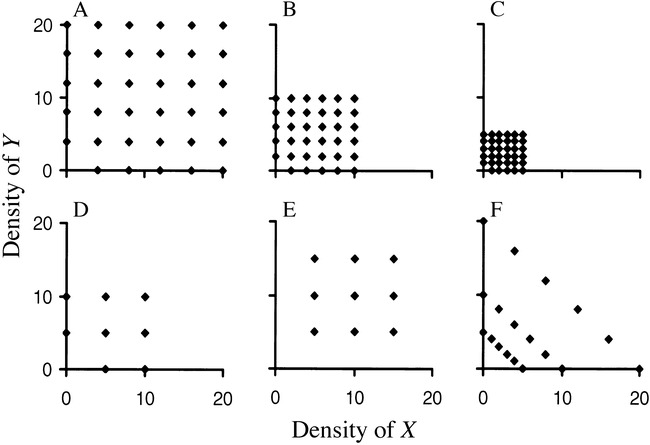
\includegraphics[width=0.5\textwidth]{..//figures/response_surface.jpg}
\caption{Example of different response surface experimental designs from Inouye, 2001.}
\label{fig:Figure 7}
\end{figure}

\end{document}
